\documentclass[11pt,final,hidelinks]{article}
\usepackage[utf8]{inputenc}
\usepackage[T1]{fontenc}
\usepackage{lmodern}
\usepackage[margin=1in]{geometry}
\usepackage[english]{babel}
\usepackage{graphicx}
\usepackage[activate={true,nocompatibility},final,tracking=true,kerning=true,spacing=true,factor=1100,stretch=10,shrink=10]{microtype}
\usepackage{mathtools}
\usepackage{amsmath}
\usepackage{amsthm}
\usepackage{amssymb}
\usepackage{booktabs}
\usepackage{hyperref}
\usepackage[square,numbers]{natbib}
\bibliographystyle{plainnat}
\usepackage{cleveref}
\usepackage{tikz}
\usetikzlibrary{arrows.meta,positioning}

% Include unified notation definitions shared across the Bernoulli series
% Unified Notation for Bernoulli Types Research
% =============================================
%
% This file provides consistent notation across all papers based on the
% latent/observed framework that is central to Bernoulli types.
%
% Core Principle: Distinguish between latent (true) and observed (noisy) values

% ========== GENERAL NOTATION ==========

% Latent values (no special decoration - these are the "true" values)
% - x, y, z for elements
% - S, T, U for sets  
% - f, g, h for functions

% Observed values (use tilde to indicate observation/approximation)
% - \obs{x}, \obs{y}, \obs{z} for observed elements
% - \obs{S}, \obs{T}, \obs{U} for observed sets
% - \obs{f}, \obs{g}, \obs{h} for observed functions

\newcommand{\obs}[1]{\widetilde{#1}}  % Universal observation operator

% Alternative: Use \latent and \observed for clarity in definitions
\newcommand{\latent}[1]{#1}
\newcommand{\observed}[1]{\widetilde{#1}}

% ========== BERNOULLI TYPES ==========

% Bernoulli type constructor: B_T^{(k)} following the refined framework
\newcommand{\BType}[1]{B_{#1}}  % Basic Bernoulli type B_T
\newcommand{\BTypeOrder}[2]{B_{#1}^{(#2)}}  % Bernoulli type with order B_T^{(k)}

% Specific Bernoulli types
\newcommand{\BBool}{B_{\mathrm{bool}}}  % Bernoulli Boolean
\newcommand{\BBoolOrder}[1]{B_{\mathrm{bool}}^{(#1)}}  % Bernoulli Boolean with order
\newcommand{\BSet}[1]{B_{#1 \mapsto \mathrm{bool}}}  % Bernoulli set (set indicator function)
\newcommand{\BMap}[2]{B_{#1 \mapsto #2}}  % Bernoulli map from type 1 to type 2

% Latent value notation - B_T(x) represents observation of latent x
\newcommand{\BValue}[2]{B_{#1}(#2)}  % B_T(x) - Bernoulli observation of latent x
\newcommand{\BValueOrder}[3]{B_{#1}^{(#2)}(#3)}  % B_T^{(k)}(x) - with explicit order

% ========== ERROR RATES ==========

% General error terminology (for any type)
\newcommand{\errorrate}{\epsilon}  % Generic error rate
\newcommand{\missrate}{\delta}     % Miss rate (fail to detect when present)
\newcommand{\spuriousrate}{\alpha} % Spurious rate (detect when absent)
\newcommand{\confusionrate}{\gamma} % Confusion between different values

% Boolean-specific terminology (only use for Boolean/binary contexts)
\newcommand{\fprate}{\alpha}  % False positive rate (Boolean only!)
\newcommand{\fnrate}{\beta}   % False negative rate (Boolean only!)
\newcommand{\tprate}{\tau}    % True positive rate (Boolean only!)
\newcommand{\tnrate}{\rho}    % True negative rate (Boolean only!)
\newcommand{\FPR}{\mathsf{FPR}}  % False positive rate (text form)
\newcommand{\FNR}{\mathsf{FNR}}  % False negative rate (text form)

% General approximation error for type T
\newcommand{\ApproxError}[2]{\epsilon_{#1 \to #2}}  % Error from type T1 to T2
\newcommand{\TypeConfusion}[3]{\gamma_{#1}(#2 \to #3)}  % Confusion in type T: value1 -> value2

% Error rate notation for specific structures
\newcommand{\withError}[3]{#1_{#2,#3}}  % e.g., \withError{S}{\spuriousrate}{\missrate}

% ========== ERROR MODEL ORDERS ==========

% Order-2 error model (uniform error rates)
\newcommand{\OrderTwo}{\text{Order-2}}
\newcommand{\UniformError}[2]{\epsilon_{#1}, \delta_{#2}}  % Uniform rates

% Order-|U| error model (element-specific error rates)
\newcommand{\OrderU}{\text{Order-}|\Universe|}
\newcommand{\ElementError}[1]{\text{error}(#1)}  % Element-specific error function
\newcommand{\ElementSpuriousRate}[1]{\spuriousrate_{#1}}   % Element-specific spurious rate
\newcommand{\ElementMissRate}[1]{\missrate_{#1}}           % Element-specific miss rate
% Boolean-specific (only use when appropriate)
\newcommand{\ElementFPRate}[1]{\fprate_{#1}}   % Element-specific false positive (Boolean only!)
\newcommand{\ElementFNRate}[1]{\fnrate_{#1}}   % Element-specific false negative (Boolean only!)

% ========== PROBABILITY AND EXPECTATION ==========

\newcommand{\Prob}[1]{\mathbb{P}\left[#1\right]}
\newcommand{\ProbCond}[2]{\mathbb{P}\left[#1 \mid #2\right]}  % Conditional probability
\newcommand{\Expect}[1]{\mathbb{E}\left[#1\right]}
\newcommand{\Var}[1]{\mathrm{Var}\left[#1\right]}

% ========== INFORMATION THEORY ==========

\newcommand{\Entropy}[1]{H(#1)}  % General entropy H(X)
\newcommand{\ConditionalEntropy}[2]{H(#1 \mid #2)}  % Conditional entropy H(X|Y)
\newcommand{\MatrixEntropy}[1]{H(#1)}  % Matrix entropy H(Q)
\newcommand{\MutualInfo}[2]{I(#1; #2)}  % Mutual information I(X;Y)
\newcommand{\KLDiv}[2]{D_{\mathrm{KL}}(#1 \parallel #2)}  % KL divergence

% ========== SET NOTATION ==========

% Basic sets
\newcommand{\Universe}{\mathcal{U}}  % Universal set
\newcommand{\PowerSet}[1]{\mathcal{P}(#1)}  % Power set
\newcommand{\EmptySet}{\emptyset}

% Set operations (no special commands needed, use standard LaTeX)
% \cup for union
% \cap for intersection  
% \setminus for difference
% \triangle for symmetric difference

% Set operations
\newcommand{\SetUnion}{\cup}
\newcommand{\SetIntersection}{\cap}
\newcommand{\SetComplement}[1]{\overline{#1}}
\newcommand{\Complement}[1]{\overline{#1}}
\newcommand{\PS}[1]{\mathcal{P}(#1)}  % Alternate power set notation

% Cardinality
\newcommand{\Card}[1]{\lvert#1\rvert}

% Membership indicator
\newcommand{\Indicator}[1]{\mathbf{1}_{#1}}

% ========== TYPE NOTATION ==========

\newcommand{\Type}[1]{\mathtt{#1}}

% ========== BOOLEAN VALUES ==========

\newcommand{\Bool}{\mathbb{B}}
\newcommand{\True}{\mathtt{true}}
\newcommand{\False}{\mathtt{false}}

% ========== CHANNEL/CONFUSION MATRIX ==========

% Channel notation: observed | latent
\newcommand{\Channel}[2]{\Prob{\text{observe } #1 \mid \text{latent } #2}}

% Confusion matrix entry
\newcommand{\Confusion}[2]{q_{#1,#2}}  % q_ij = P(observe j | latent i)

% ========== FUNCTION NOTATION ==========

% Function composition (use standard \circ)
% Approximate/observed function application
\newcommand{\ApproxApply}[2]{\obs{#1}(#2)}  % \ApproxApply{f}{x}

% ========== USAGE EXAMPLES ==========

% Example 1: Bernoulli Boolean
% Latent: x \in \Bool
% Observed: \obs{x} \in \Bernoulli{\Bool}{2}
% Relationship: \Channel{\obs{x} = \True}{x = \False} = \fprate

% Example 2: Bernoulli Set  
% Latent: S \subseteq U
% Observed: \obs{S} observes S with rates (\fprate, \fnrate)
% Query: \Channel{x \in \obs{S}}{x \notin S} = \fprate

% Example 3: Composition
% Latent: f \circ g
% Observed: \obs{f} \circ \obs{g}
% Error: \errorrate_{\obs{f} \circ \obs{g}} = \errorrate_f + \errorrate_g - \errorrate_f \errorrate_g

% ========== DEPRECATED NOTATION ==========
% The following should be replaced:
% \ASet{S} → \obs{S}
% \PASet{S} → \obs{S}^+ or \withError{S}{\fprate}{0}  
% \NASet{S} → \obs{S}^- or \withError{S}{0}{\fnrate}
% \Set{S} → S (no decoration needed for latent)

% ========== NOTATION TABLE (for inclusion) ==========

\newcommand{\BernoulliNotationTable}{%
\begin{tabular}{@{}ll@{}}
\textbf{Symbol} & \textbf{Meaning} \\
\midrule
$\obs{x}$ & Observed value corresponding to latent $x$ \\
$\obs{S}$ & Observed (approximate) set for latent $S$ \\
$\obs{f}$ & Observed map approximating latent $f$ \\
$\spuriousrate$ & Spurious rate: $\Prob\{\obs{x}\in\obs{S} \mid x\notin S\}$ \\
$\missrate$ & Miss rate: $\Prob\{\obs{x}\notin\obs{S} \mid x\in S\}$ \\
$\confusionrate$ & Confusion rate between different values \\
$\ElementError{x}$ & Element-specific error function for $x$ \\
$\ElementSpuriousRate{x}$ & Spurious rate specific to element $x$ \\
$\ElementMissRate{x}$ & Miss rate specific to element $x$ \\
$\errorrate$ & Generic error rate $\Prob\{\obs{f}(x)\neq f(x)\}$ \\
$\ApproxError{T_1}{T_2}$ & Approximation error from type $T_1$ to $T_2$ \\
$\TypeConfusion{T}{v_1}{v_2}$ & Confusion in type $T$: value $v_1 \to v_2$ \\
$\fprate, \fnrate$ & False pos./neg. rates (Boolean contexts only) \\
$Q$ & Confusion matrix: $Q_{ij}=\Prob\{\text{obs } t_j\mid \text{lat } t_i\}$ \\
$W(y\mid x)$ & Channel kernel from latent $x$ to observed $y$ \\
$\Entropy{Q}$ & Matrix entropy of confusion matrix $Q$ \\
$\ConditionalEntropy{\text{lat}}{\text{obs}}$ & Conditional entropy of latent given observed \\
$\MutualInfo{X}{Y}$ & Mutual information between $X$ and $Y$ \\
$\Indicator{S}$ & Set indicator function $U\to\Bool$ \\
$\Complement{S}$ & Set complement \\
$\Card{S}$ & Cardinality of a set $S$ \\
\end{tabular}%
}

\newcommand{\NotationSection}{%
\section*{Notation}
This section summarizes symbols used throughout the paper. See also the shared cheat sheet for formulas and assumptions.

\medskip
\noindent\BernoulliNotationTable
}


% Theorem environments
\newtheorem{theorem}{Theorem}[section]
\newtheorem{lemma}[theorem]{Lemma}
\newtheorem{proposition}[theorem]{Proposition}
\newtheorem{corollary}[theorem]{Corollary}
\newtheorem{definition}[theorem]{Definition}
\newtheorem{example}[theorem]{Example}
\newtheorem{remark}[theorem]{Remark}
\newtheorem{axiom}{Axiom}

% Custom commands for algebraic data types and X± notation
\newcommand{\bernoulli}[2]{\mathcal{B}\langle #1, #2 \rangle}
\newcommand{\powerset}[1]{\mathcal{P}(#1)}
\newcommand{\xpm}{X^{\pm}} % X± notation for approximate types
\newcommand{\voidtype}{\mathsf{Void}}
\newcommand{\unittype}{\mathsf{Unit}}
\newcommand{\sumtype}[2]{#1 + #2}
\newcommand{\prodtype}[2]{#1 \times #2}
\newcommand{\exptype}[2]{#1 \to #2}
\newcommand{\approxmap}[3]{#1 \xrightarrow{#2}_{#3} #2} % X →^ε_ω Y notation

\title{Foundations of Bernoulli Types: A Probabilistic Framework for Data Structures and Types}
\author{
    Alexander Towell\\
    \texttt{atowell@siue.edu}
}
\date{\today}

\begin{document}
\maketitle
\NotationSection

\begin{abstract}
We introduce the \emph{Bernoulli Model}, a probabilistic framework that systematically handles uncertainty in data structures and types. The Boolean type $\mathrm{bool}$ is replaced with $B_{\mathrm{bool}}$, representing a noisy Boolean, and this extends to any type $T$ with $B_T$. Each Bernoulli type has an \emph{order} $k$ denoted $B_T^{(k)}$, representing degrees of freedom in error modeling. The framework operates at two levels: crystallized instances ($B_{\mathrm{bool}}$, $B_{X \mapsto Y}$, $B_{X \mapsto \mathrm{bool}}$) that capture essential patterns, and general algebraic foundations showing how approximation composes through type constructors. Central to the framework are confusion matrices characterizing latent-observed relationships, enabling space-accuracy trade-offs with $\mathcal{O}(1)$ time complexity. We demonstrate that Bloom filters, Count-Min sketches, and randomized algorithms are instances of this systematic approach, providing both theoretical foundations for error propagation and practical implementation guidance for oblivious data structures.
\end{abstract}

\section{Introduction}

\subsection{The Fundamental Problem: Observing the Unobservable}

In many computational contexts, we cannot directly access the values we care about. Instead, we work with noisy observations:

\begin{itemize}
    \item A Bloom filter stores a \emph{latent} set $S$, but we can only \emph{observe} membership queries that may have false positives
    \item A sketch maintains a \emph{latent} frequency distribution, but we can only \emph{observe} approximate counts
    \item A randomized algorithm computes a \emph{latent} result, but we can only \emph{observe} a probabilistic output
    \item A compressed data structure represents \emph{latent} information, but we can only \emph{observe} lossy reconstructions
\end{itemize}

This paper formalizes the relationship between latent values and their observations through \emph{Bernoulli types}—a type system where approximation is a first-class concept.

Consider the ubiquitous Bloom filter, which provides approximate set membership queries with one-sided error. While traditionally viewed as a specialized data structure, we show that it is merely one instance of a much broader class of Bernoulli types. By lifting approximation to the type level, we can reason about error propagation through complex systems in a principled manner.

\paragraph{Scope and organization.}  This article is the first in a series exploring Bernoulli types and the latent/observed paradigm.  Here we introduce the foundations: the basic definitions, the channel interpretation, and the core theorems.  Subsequent papers build on these ideas.  In \textbf{Part~2} we develop the algebra of Bernoulli sets and derive how set operations propagate observation error.  \textbf{Part~3} introduces Bernoulli maps as a universal framework for approximate functions.  \textbf{Part~4} examines how the notion of a ``regular'' type must be revised when equality is itself observed through a noisy channel.  \textbf{Part~5} applies Bernoulli sets to information retrieval and Boolean search.  \textbf{Part~6} describes space–optimal implementations using entropy coding, and \textbf{Part~7} provides a statistical analysis of the distributions and confidence intervals that arise when observing finite sets.

\paragraph{Connection to oblivious computing.} The rank-based analysis developed here provides fundamental insights into \emph{oblivious computing} and privacy-preserving computation. When privacy constraints are imposed on observable information, they manifest as rank-deficiency in confusion matrices, creating asymptotic indistinguishability bounds that persist regardless of computational resources. This connection forms the theoretical foundation for our companion \textbf{Oblivious Series}, which explores how Bernoulli approximations enable privacy-preserving data structures, secure multi-party computation protocols, and differential privacy mechanisms while maintaining the utility-privacy trade-offs predicted by the rank-based framework developed here.

\subsection{Motivating Examples}

Before formalizing the framework, we present three motivating examples that showcase different aspects of Bernoulli types:

\begin{example}[Approximate Boolean]
The simplest non-trivial Bernoulli type is the approximate Boolean. Given a latent Boolean value $x \in \{\True, \False\}$, an observation $\tilde{x} \in \bernoulli{\Bool}{1}$ may differ from $x$ with probability $p$. This models a binary symmetric channel where the observed value is a noisy version of the latent truth.
\end{example}

\begin{example}[Bloom Filter as Bernoulli Set]
A Bloom filter stores a latent set $S \subseteq U$ but only allows observations through membership queries. For any element $u \in U$, the observation "$u \in? S$" has:
\begin{itemize}
    \item If $u \in S$ (latent): always observes "yes" (no false negatives)
    \item If $u \notin S$ (latent): may observe "yes" with probability $\alpha$ (false positives)
\end{itemize}
\end{example}

\begin{example}[Miller-Rabin as Bernoulli Map]
The Miller-Rabin primality test observes the latent property "is $n$ prime?" through randomized testing. Given latent truth $\text{isPrime}(n)$, the observed result:
\begin{itemize}
    \item If $n$ is prime (latent): always observes "prime" 
    \item If $n$ is composite (latent): may observe "prime" with probability $\leq 1/4^k$
\end{itemize}
\end{example}

\section{The Bernoulli Model: From Concrete to General}

The Bernoulli Model provides a systematic framework for approximation that operates at two levels: specific crystallized instances and general algebraic foundations. We begin with the concrete and build toward the general.

\subsection{Crystallized Instances}

The framework is best understood through key crystallized cases that capture the essential patterns:

\begin{definition}[Bernoulli Boolean]
The Boolean type $\mathrm{bool} = \{\mathrm{true}, \mathrm{false}\}$ is replaced with $\BBool$, representing a noisy Boolean. A value $\BValue{\mathrm{bool}}{x}$ represents a Bernoulli observation of latent Boolean $x$, where:
$$\Pr\{\BValue{\mathrm{bool}}{x} \neq x\} = \text{Error}(x)$$
\end{definition}

\begin{definition}[Bernoulli Order]
Each Bernoulli type has an \emph{order} $k$ denoted $\BTypeOrder{T}{k}$, representing degrees of freedom in the error model:
\begin{itemize}
    \item \textbf{Order-0}: Deterministic, $\BTypeOrder{T}{0} \equiv T$
    \item \textbf{Order-1}: Symmetric errors (binary symmetric channel)
    \item \textbf{Order-2+}: Asymmetric error patterns
\end{itemize}
\end{definition}

\begin{definition}[Bernoulli Maps]
Functions $f: X \to Y$ have latent values we approximate with $\BMap{X}{Y}$. The observed function $\BValue{X \to Y}{f}$ produces outputs of type $\BType{Y}$, capturing uncertainty in both function identity and output values.
\end{definition}

\begin{definition}[Bernoulli Sets]
Set-indicator functions $1_S: X \to \mathrm{bool}$ are approximated as $\BSet{X}$. This captures data structures like Bloom filters as Bernoulli approximations of membership testing.
\end{definition}

\subsection{Algebraic Foundations}

These crystallized instances arise from systematic application of Bernoulli approximation to algebraic data types:

\begin{definition}[Algebraic Data Types]
Types are built compositionally from:
\begin{itemize}
    \item \textbf{Void type} ($\voidtype$): Empty type, $\BType{\voidtype} = \voidtype$
    \item \textbf{Unit type} ($\unittype$): Singleton type, $\BType{\unittype} = \unittype$ 
    \item \textbf{Sum type} ($X + Y$): Disjoint union
    \item \textbf{Product type} ($X \times Y$): Cartesian product  
    \item \textbf{Exponential type} ($X \to Y$): Function type
\end{itemize}
\end{definition}

\begin{definition}[Compositional vs Direct Approximation]
For compound types, there are two approximation approaches:
\begin{itemize}
    \item \textbf{Compositional}: $(\BType{X}, \BType{Y})$ - approximate components first
    \item \textbf{Direct}: $\BType{X \times Y}$ - approximate the compound type directly
\end{itemize}
Both are valid Bernoulli types with different error characteristics.
\end{definition}

This systematic relationship between crystallized instances and algebraic foundations provides both practical guidance and theoretical completeness.

\subsection{Confusion Matrices: The Core Formalism}

Every Bernoulli type is characterized by a confusion matrix that describes the probability relationship between latent and observed values.

\begin{definition}[Confusion Matrix]
For a Bernoulli type $\BType{T}$ where $T = \{t_1, t_2, \ldots, t_n\}$, the confusion matrix $Q$ has entries:
$$q_{ij} = \Pr\{\text{observe } t_j \mid \text{latent } t_i\}$$
where each row sums to 1: $\sum_{j=1}^n q_{ij} = 1$.
\end{definition}

\begin{example}[Bernoulli Boolean Confusion Matrix]
For $\BBoolOrder{2}$ (second-order), we have:

\begin{center}
\begin{tabular}{c|cc}
latent $\backslash$ observed & $\mathrm{true}$ & $\mathrm{false}$ \\
\hline
$\mathrm{true}$ & $1-\eta$ & $\eta$ \\
$\mathrm{false}$ & $\varepsilon$ & $1-\varepsilon$ \\
\end{tabular}
\end{center}

Where $\eta$ is the false negative rate and $\varepsilon$ is the false positive rate. This has 2 degrees of freedom, hence order-2.
\end{example}

\begin{example}[Bernoulli Function Confusion Matrix]
For functions $f: \mathrm{bool} \to \mathrm{bool}$, there are 4 possible functions $\{\mathrm{id}, \mathrm{not}, \mathrm{true}, \mathrm{false}\}$. The confusion matrix for $\BMap{\mathrm{bool}}{\mathrm{bool}}$ is:

\begin{center}
\begin{tabular}{c|cccc}
latent $\backslash$ observed & $\mathrm{id}$ & $\mathrm{not}$ & $\mathrm{true}$ & $\mathrm{false}$ \\
\hline
$\mathrm{id}$ & $q_{11}$ & $q_{12}$ & $q_{13}$ & $q_{14}$ \\
$\mathrm{not}$ & $q_{21}$ & $q_{22}$ & $q_{23}$ & $q_{24}$ \\
$\mathrm{true}$ & $q_{31}$ & $q_{32}$ & $q_{33}$ & $q_{34}$ \\
$\mathrm{false}$ & $q_{41}$ & $q_{42}$ & $q_{43}$ & $q_{44}$ \\
\end{tabular}
\end{center}

Maximum order is $4(4-1) = 12$ degrees of freedom.
\end{example}

\begin{definition}[Order of Bernoulli Type]
The order of $\BTypeOrder{T}{k}$ is the number of free parameters in its confusion matrix. For type $T$ with $n$ values, the maximum order is $n(n-1)$ since each row must sum to 1.
\end{definition}

\begin{definition}[Rank of Bernoulli Type]
The \emph{rank} of a Bernoulli type is the matrix rank of its confusion matrix. This captures the fundamental degrees of freedom in the probability space and determines the theoretical limits of Bayesian inference.
\end{definition}

\begin{remark}[Order vs Rank]
Order and rank capture different aspects of Bernoulli approximations:
\begin{itemize}
    \item \textbf{Order (parameter count)}: Affects estimation difficulty from data
    \item \textbf{Rank}: Determines fundamental inferability of latent from observed values
\end{itemize}
A confusion matrix can have low rank despite high order, making Bayesian inference $\Prob\{\text{latent} \mid \text{observed}\} \propto \Prob\{\text{observed} \mid \text{latent}\} \Prob\{\text{latent}\}$ impossible even with perfect parameter estimates.
\end{remark}

\begin{example}[Rank Analysis for Bernoulli Boolean]
For $\BBoolOrder{1}$ with error rate $\varepsilon$:
\begin{itemize}
    \item Order = 1, Rank = 2 for $\varepsilon \neq 0.5$ (invertible, inference possible)
    \item Order = 1, Rank = 1 for $\varepsilon = 0.5$ (singular, inference impossible)
\end{itemize}
The rank-1 case corresponds to maximum entropy where observations provide no information about latent values.
\end{example}

\begin{remark}[Asymptotic Indistinguishability and Oblivious Computing]
Rank provides fundamental asymptotic limits that persist even with perfect parameter knowledge. When a confusion matrix has rank $r < n$ (where $n$ is the number of possible latent values), then $n-r$ degrees of freedom become \emph{asymptotically indistinguishable} regardless of:
\begin{itemize}
    \item Sample size (even with infinite observations)
    \item Parameter estimation accuracy (even with perfect confusion matrix knowledge)
    \item Computational resources (even with unlimited processing power)
\end{itemize}

This connects directly to \emph{oblivious computing} where privacy constraints manifest as structural rank-deficiency in observable information. The rank determines \emph{information-theoretic privacy bounds} that no algorithm can overcome—certain latent information remains fundamentally hidden by the mathematical structure of the approximation process itself.
\end{remark}

\subsection{Information-Theoretic Perspective}

Entropy provides a third fundamental measure of Bernoulli approximations, complementing order and rank.

\begin{definition}[Matrix Entropy]
The \emph{matrix entropy} of a confusion matrix $Q$ is:
$$H(Q) = -\sum_{i,j} q_{ij} \log q_{ij}$$
This measures the uncertainty in the approximation process itself.
\end{definition}

\begin{definition}[Conditional Entropy]
The \emph{conditional entropy} $H(\text{latent} \mid \text{observed})$ measures remaining uncertainty about latent values given observations, computed via Bayesian inference.
\end{definition}

\begin{theorem}[Information Hierarchy]
Knowledge constraints reduce entropy in a hierarchical manner:
\begin{enumerate}
    \item \textbf{Unconstrained}: Maximum entropy over all possible confusion matrices
    \item \textbf{Structural constraints}: Entropy reduced by algorithm-specific structure (e.g., ``Bloom filter'')  
    \item \textbf{Parameter knowledge}: Further reduction by known parameter values
    \item \textbf{Observations}: Conditional entropy given observed values
\end{enumerate}
Each level provides additional information that reduces uncertainty.
\end{theorem}

\begin{example}[Confusion Matrix Scales]
Confusion matrices operate at two scales:

\textbf{Small Types}: For $\BBool$, the $2 \times 2$ confusion matrix can be written explicitly and analyzed completely.

\textbf{Large Types}: For $\BSet{U}$ (Bernoulli sets), the confusion matrix has $2^{|U|} \times 2^{|U|}$ entries, typically too large to write explicitly. However, \emph{structural patterns} still determine fundamental limits.
\end{example}

\begin{example}[Bloom Filter Structural Analysis]
A Bloom filter has a $2^{|U|} \times 2^{|U|}$ confusion matrix with:
\begin{itemize}
    \item \textbf{Sparsity structure}: $\Prob\{\text{observe } T \mid \text{latent } S\} = 0$ when $T \not\subseteq S$
    \item \textbf{High rank}: Effective rank $\approx 2^{|S|}$ due to subset preservation creating identity-like blocks
    \item \textbf{Enhanced inference}: Structure enables better inference than random matrices
\end{itemize}

\textbf{Individual membership query}: Each query produces a Bernoulli bool with $2 \times 2$ matrix:
$$Q = \begin{pmatrix} 1 & 0 \\ \varepsilon & 1-\varepsilon \end{pmatrix}$$
\end{example}

\section{Error Model Hierarchies}

Before formalizing Bernoulli types, we must distinguish between different orders of error models that can arise in approximate computation.

\subsection{Order-2 vs Order-|U| Error Models}

\begin{definition}[General Error Function]
For any type $T$, the \emph{error function} for element $x \in T$ is:
$$\text{Error}(x) = \Prob\{\obs{x} \neq x\}$$
This captures the fundamental notion that the observed value differs from the latent value.
\end{definition}

\begin{definition}[Order-2 Error Model]
In an \emph{order-2 error model}, there are exactly two uniform error parameters. Different systems use varying terminology:
\begin{itemize}
    \item \textbf{Set membership}: spurious rate $\spuriousrate$ (detect when absent), miss rate $\missrate$ (miss when present)
    \item \textbf{Boolean classification}: false positive rate $\fprate$, false negative rate $\fnrate$ 
    \item \textbf{Information theory}: type I error, type II error
    \item \textbf{Signal processing}: false alarm rate, miss detection rate
\end{itemize}
The key property is uniformity: $\text{Error}(x) = \epsilon$ for all $x$.
\end{definition}

\begin{definition}[Order-|U| Error Model]
In an \emph{order-|U| error model}, each element has its own error characteristics:
$$\text{Error}(x) = \epsilon_x \quad \text{for each } x \in U$$
This allows $|U|$ distinct error parameters. While maximally general, it is typically intractable for analysis and implementation.
\end{definition>

\begin{remark}[Algorithmic Preference for Order-2]
While the order-|U| model provides greater theoretical generality, the order-2 model dominates in practice because:
\begin{itemize}
    \item Most algorithms that compute representations of approximate sets (Bloom filters, sketches, etc.) naturally produce uniform error rates
    \item Order-2 models are tractable for analysis and composition
    \item Storage and computational complexity remain manageable
    \item The uniform error assumption often approximates real-world behavior sufficiently well
\end{itemize}
\end{remark}

\begin{example}[Hash-Based Structures]
Consider a Bloom filter with $k$ hash functions and $m$ bits. The false positive probability $\varepsilon = (1 - e^{-kn/m})^k$ is uniform across all queries, naturally yielding an order-2 model. While individual elements might have slightly different collision patterns, the design ensures approximately uniform behavior.
\end{example}

\begin{example}[Element-Specific Errors]
An order-|U| model might arise when:
\begin{itemize}
    \item Elements have different hash qualities leading to varying collision rates
    \item Approximate data structures adapt their precision based on element frequency
    \item Physical constraints (memory locality, cache behavior) create element-dependent errors
\end{itemize}
\end{example}

Throughout this series, we primarily focus on order-2 models while noting where the framework naturally extends to higher-order cases.

\section{Mathematical Foundations of Bernoulli Types}

\subsection{Basic Definitions}

\begin{definition}[Latent and Observed Values]
For any type $T$:
\begin{itemize}
    \item A \emph{latent value} $x \in T$ represents the true, unobservable value
    \item An \emph{observed value} $\tilde{x} \in \bernoulli{T}{n}$ represents a noisy observation of some latent value
\end{itemize}
We write $\tilde{x} \sim \bernoulli{T}{n}(x)$ to denote that $\tilde{x}$ is an observation of latent value $x$.
\end{definition}

\begin{definition}[Bernoulli Type Constructor]
Given an algebraic data type $T$, the Bernoulli type constructor $\bernoulli{T}{n}$ produces a type whose values are observations of latent values in $T$. This constructor satisfies:
\begin{itemize}
    \item $\bernoulli{T}{n}$ is equivalent to $T^{\pm}$ in the X$^{\pm}$ notation
    \item Observations are related to their latent values through an $n$-th order error model
    \item The constructor respects the algebraic structure: $\bernoulli{(\sumtype{X}{Y})}{n} \cong \sumtype{\bernoulli{X}{n}}{\bernoulli{Y}{n}}$
\end{itemize}
\end{definition}

\begin{remark}[Connection to Algebraic Data Types]
The Bernoulli type constructor can be applied systematically to any algebraic data type:
\begin{itemize}
    \item $\bernoulli{\voidtype}{n} = \voidtype$ (no approximation possible for empty type)
    \item $\bernoulli{\unittype}{n} = \unittype$ (no approximation needed for singleton)  
    \item $\bernoulli{(\sumtype{X}{Y})}{n}$ allows approximate discrimination between variants
    \item $\bernoulli{(\prodtype{X}{Y})}{n}$ allows approximate access to components
    \item $\bernoulli{(\exptype{X}{Y})}{n}$ represents approximate functions (random approximate maps)
\end{itemize}
\end{remark}

The order $n$ specifies the complexity of the error model:
\begin{itemize}
    \item $n = 0$: Perfect observation (no errors, $\tilde{x} = x$ always)
    \item $n = 1$: Symmetric errors (observation errors independent of latent value)
    \item $n = 2$: Asymmetric errors (observation errors depend on latent value class)
    \item $n > 2$: Element-specific errors (observation errors depend on specific latent value)
\end{itemize}

\begin{definition}[Observation Distribution]
For a Bernoulli type $\bernoulli{T}{n}$ with error profile $\sigma$, the observation distribution specifies:
\begin{equation}
\Prob{\tilde{x} = y | x} = P_\sigma(y|x)
\end{equation}
where $x$ is the latent value and $y$ is the observed value.
\end{definition}

\subsection{Channel Model Interpretation}

Bernoulli types can be understood through the lens of information theory as noisy channels:

\begin{theorem}[Channel Correspondence]
Every Bernoulli type $\bernoulli{T}{n}$ with error profile $\sigma$ corresponds to a discrete memoryless channel with input alphabet $T$, output alphabet $T$, and transition probabilities determined by $\sigma$.
\end{theorem}

\begin{figure}[t]
\centering
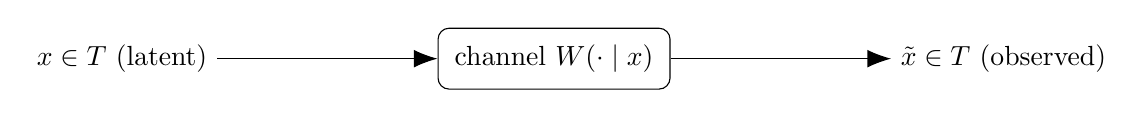
\begin{tikzpicture}[node distance=2.8cm]
  \node (X) {$x\in T$ (latent)};
  \node (chan) [right=of X, draw, rounded corners, inner sep=6pt] {channel $W(\cdot\mid x)$};
  \node (Y) [right=of chan] {$\tilde{x}\in T$ (observed)};
  \draw[-{Latex[length=3mm]}] (X) -- (chan);
  \draw[-{Latex[length=3mm]}] (chan) -- (Y);
\end{tikzpicture}
\caption{Latent-to-observed channel view of Bernoulli types.}
\end{figure}

\subsection{Order and Confusion Matrices}

For a finite type $T=\{t_1,\dots,t_m\}$, the \emph{confusion matrix} $Q\in[0,1]^{m\times m}$ of a Bernoulli type records
\begin{equation}
    Q_{ij} \coloneqq \Prob{\text{observe } t_j \mid \text{latent } t_i}, \qquad \sum_{j=1}^m Q_{ij}=1.
\end{equation}
We define the \emph{order} of a Bernoulli type on $T$ as the number of independent error parameters, i.e., the degrees of freedom in $Q$ off the identity. In the extreme, a symmetric model has a single parameter $\epsilon$ with
\begin{equation}
    Q_{ij}=\begin{cases}1-\epsilon,& i=j,\\[2pt] \epsilon/(m-1),& i\neq j.\end{cases}
\end{equation}
For $T=\Bool$, the second-order (asymmetric) model splits errors into false positives $\fprate$ and false negatives $\fnrate$:
\begin{center}
\begin{tabular}{c|cc}
latent $\backslash$ observed & $\True$ & $\False$ \\ \hline
$\True$ & $1-\fnrate$ & $\fnrate$ \\
$\False$ & $\fprate$ & $1-\fprate$
\end{tabular}
\end{center}

\subsection{Bayesian Inference and Multiple Observations}

Let $\tilde{x}\sim\bernoulli{T}{n}(x)$ be an observation and let $\pi$ be a prior on $T$. For finite $T$, Bayes' rule yields
\begin{equation}
    \Prob{x=t_i\mid \tilde{x}=t_j} = \frac{Q_{ij}\,\pi(t_i)}{\sum_{r=1}^m Q_{rj}\,\pi(t_r)}.
\end{equation}
If we obtain i.i.d. observations $\tilde{x}_1,\dots,\tilde{x}_k$ under a memoryless channel, the joint likelihood factorizes and the posterior concentrates around the latent value. In the Boolean case with symmetric error $\epsilon<\tfrac12$, the majority vote of $k$ observations is a consistent estimator and the error probability decays exponentially in $k$ (Chernoff/Hoeffding bounds).

\subsection{Approximate Value Monad}

The X$^{\pm}$ framework naturally leads to a monadic structure for composing approximate computations.

\begin{definition}[Approximate Value Monad]
The approximate value monad $\mathsf{Approx}(X)$ encapsulates values of type $X^{\pm}$ together with their error characteristics:
\begin{itemize}
    \item $\mathsf{return}: X \to \mathsf{Approx}(X)$ embeds exact values with zero error
    \item $\mathsf{bind}: \mathsf{Approx}(X) \times (X \to \mathsf{Approx}(Y)) \to \mathsf{Approx}(Y)$ composes approximate computations
\end{itemize}
\end{definition}

Given a function $f: X \to Y$ and an approximate value $\tilde{x} \in \mathsf{Approx}(X)$, the lifted function $\tilde{f}: \mathsf{Approx}(X) \to \mathsf{Approx}(Y)$ propagates uncertainty according to:
\begin{equation}
\tilde{f}(\tilde{x}) = \mathsf{bind}(\tilde{x}, \lambda x. \mathsf{return}(f(x)))
\end{equation}

This monadic structure enables systematic error propagation through complex computations while maintaining the algebraic properties of the underlying types.

\begin{remark}[Type Erasure]
The concrete error parameters of approximate types can be erased for modularity. A value $f^{\omega}_{\varepsilon}$ with specific error rates can be erased to $f^{\pm}$ (generic approximate function) or further to $f$ (hiding approximation entirely).
\end{remark}

\begin{proof}
We establish a bijection between Bernoulli types and discrete memoryless channels (DMCs).

\textbf{Forward direction:} Given $\bernoulli{T}{n}$ with error profile $\sigma$, construct a DMC as follows:
\begin{itemize}
    \item Input alphabet: $\mathcal{X} = T$
    \item Output alphabet: $\mathcal{Y} = T$
    \item Channel matrix: $W(y|x) = P_\sigma(y|x)$ where $P_\sigma$ is determined by the error profile
\end{itemize}

For order $n = 1$ (symmetric), we have:
\begin{equation}
W(y|x) = \begin{cases}
1 - \epsilon & \text{if } y = x \\
\frac{\epsilon}{|T| - 1} & \text{if } y \neq x
\end{cases}
\end{equation}

For order $n = 2$ (asymmetric), partition $T = T_+ \cup T_-$ and:
\begin{equation}
W(y|x) = \begin{cases}
1 - \alpha & \text{if } x \in T_-, y = x \\
\alpha & \text{if } x \in T_-, y \in T_+ \\
1 - \beta & \text{if } x \in T_+, y = x \\
\beta & \text{if } x \in T_+, y \in T_-
\end{cases}
\end{equation}

\textbf{Reverse direction:} Given a DMC with $W(y|x)$, construct $\bernoulli{T}{n}$ by:
\begin{enumerate}
    \item Determine the order $n$ from the rank of $W - I$ where $I$ is the identity matrix
    \item Extract error parameters from the eigenvalues of $W$
    \item Define the error profile $\sigma$ from the channel transition probabilities
\end{enumerate}

\textbf{Memoryless property:} The independence axiom of Bernoulli types ensures:
\begin{equation}
P(y_1, \ldots, y_k | x_1, \ldots, x_k) = \prod_{i=1}^k P(y_i | x_i)
\end{equation}

This completes the correspondence.
\end{proof}

\subsection{Confusion Matrix Representation}

The channel correspondence naturally leads to a confusion matrix representation for Bernoulli types. For a type $T$ with $|T| = n$ elements, the confusion matrix $Q \in \mathbb{R}^{n \times n}$ captures the complete error behavior:

\begin{definition}[Confusion Matrix]
For a Bernoulli type $\bernoulli{T}{k}$, the confusion matrix $Q = [q_{ij}]$ is defined by:
\begin{equation}
q_{ij} = \Prob{\text{observe } t_j | \text{latent } t_i}
\end{equation}
where $t_1, \ldots, t_n$ enumerate the elements of $T$.
\end{definition}

\begin{example}[Boolean Confusion Matrix]
For $\bernoulli{\Bool}{2}$ with false positive rate $\alpha$ and false negative rate $\beta$:
\begin{figure}[t]
\centering
\begin{tabular}{c|cc}
latent \textbackslash observed & $\mathtt{true}$ & $\mathtt{false}$ \\
\hline
$\mathtt{true}$ & $1-\beta$ & $\beta$ \\
$\mathtt{false}$ & $\alpha$ & $1-\alpha$
\end{tabular}
\caption{Boolean asymmetric confusion matrix (BAC model).}
\end{figure}
This directly corresponds to a binary asymmetric channel (BAC).
\end{example}

\begin{proposition}[Confusion Matrix Properties]
For any Bernoulli type confusion matrix $Q$:
\begin{enumerate}
    \item \textbf{Stochasticity:} Each row sums to 1: $\sum_j q_{ij} = 1$
    \item \textbf{Order determination:} The order $k$ satisfies $k \leq n(n-1)$
    \item \textbf{Symmetry detection:} Order 1 iff $q_{ij} = \epsilon/(n-1)$ for all $i \neq j$
    \item \textbf{Accuracy measure:} Overall accuracy = $\text{tr}(Q)/n$
\end{enumerate}
\end{proposition}

\subsection{Bayesian Inference: From Observed to Latent}

The fundamental computational problem with Bernoulli types is inferring properties of latent values from observations:

\begin{theorem}[Bayesian Inference for Bernoulli Types]
Given an observation $\tilde{x} = y$ from $\bernoulli{T}{n}$, the posterior probability of the latent value is:
\begin{equation}
\Prob{x = t_i | \tilde{x} = t_j} = \frac{q_{ij} \cdot \Prob{x = t_i}}{\sum_{k=1}^{|T|} q_{kj} \cdot \Prob{x = t_k}}
\end{equation}
where $q_{ij}$ is the confusion matrix entry and $\Prob{x = t_i}$ is the prior probability.
\end{theorem}

\begin{example}[Boolean Inference]
For $\bernoulli{\Bool}{2}$ with uniform prior $\Prob{x = \True} = 0.5$:
\begin{align}
\Prob{x = \True | \tilde{x} = \True} &= \frac{1-\beta}{1-\beta + \alpha} \\
\Prob{x = \False | \tilde{x} = \False} &= \frac{1-\alpha}{1-\alpha + \beta}
\end{align}
This shows how observation quality depends on both error rates.
\end{example}

\begin{corollary}[Multiple Independent Observations]
Given $n$ independent observations $\tilde{x}_1, \ldots, \tilde{x}_n$ of the same latent value:
\begin{equation}
\Prob{x = t | \tilde{x}_1, \ldots, \tilde{x}_n} \propto \Prob{x = t} \prod_{i=1}^n \Prob{\tilde{x}_i | x = t}
\end{equation}
As $n \to \infty$, the posterior concentrates on the true latent value (assuming non-degenerate confusion matrix).
\end{corollary}

\section{The Bernoulli Type Hierarchy}

\subsection{Order 0: Deterministic Types}

When $n = 0$, we have $\bernoulli{T}{0} \cong T$. This represents the degenerate case where no approximation occurs, corresponding to a perfect channel with zero error rate.

\subsection{Order 1: Symmetric Error Models}

First-order Bernoulli types model situations where observation errors occur with equal probability regardless of the latent value:

\begin{equation}
\Prob{\tilde{x} \neq x} = \epsilon \quad \forall x \in T
\end{equation}

where $\tilde{x} \sim \bernoulli{T}{1}(x)$ is an observation of latent value $x$. This corresponds to a symmetric noisy channel where all values are equally difficult to observe accurately.

\subsection{Order 2: Asymmetric Error Models}

Second-order types distinguish between different kinds of observation errors based on the latent value. For Boolean types:

\begin{align}
\Prob{\tilde{x} = \False | x = \True} &= \beta \quad \text{(false negative rate)} \\
\Prob{\tilde{x} = \True | x = \False} &= \alpha \quad \text{(false positive rate)}
\end{align}

This asymmetry is crucial for modeling real-world systems:
\begin{itemize}
    \item Bloom filters: $\beta = 0$ (never miss latent members)
    \item Medical tests: often $\alpha \ll \beta$ (minimize false alarms)
    \item Security systems: often $\beta \ll \alpha$ (minimize missed threats)
\end{itemize}

\subsection{Higher Orders: Element-Specific Errors}

For orders $n > 2$, error rates can depend on the specific element being approximated. This models situations where certain values are more difficult to represent accurately than others.

The confusion matrix for higher-order models can have arbitrary transition probabilities, subject only to the stochastic constraint. The maximum order for a type $T$ with $|T| = m$ elements is $m(m-1)$, representing the degrees of freedom in a stochastic matrix.

\begin{example}[Function Type Maximum Order]
For $\Bool \to \Bool$, there are 4 possible functions:
\begin{itemize}
    \item $\mathtt{id}$: identity function  
    \item $\mathtt{not}$: negation
    \item $\mathtt{true}$: constant true
    \item $\mathtt{false}$: constant false
\end{itemize}
The confusion matrix is $4 \times 4$, giving maximum order $4 \times 3 = 12$. This allows modeling scenarios where, for instance, observing $\mathtt{id}$ as $\mathtt{not}$ has different probability than observing $\mathtt{true}$ as $\mathtt{false}$.
\end{example}

\subsection{Lifting Functions to Bernoulli Types}

An important operation is lifting deterministic functions to operate on Bernoulli types:

\begin{definition}[Monadic Lift]
Given $f: A \to B$, the lifted function $\tilde{f}: \bernoulli{A}{n} \to \bernoulli{B}{m}$ propagates uncertainty:
\begin{equation}
\Prob{\tilde{f}(\tilde{a}) = b | a} = \sum_{a' \in A} \Prob{\tilde{a} = a' | a} \cdot \mathbf{1}_{f(a') = b}
\end{equation}
\end{definition}

\begin{example}[Identity Function on Noisy Input]
When $\mathtt{id}: \Bool \to \Bool$ receives $\tilde{x} \in \bernoulli{\Bool}{1}$ with error rate $\epsilon$:
\begin{itemize}
    \item If latent $x = \True$: outputs $\True$ with probability $1-\epsilon$
    \item If latent $x = \False$: outputs $\False$ with probability $1-\epsilon$
\end{itemize}
Thus $\mathtt{id}: \bernoulli{\Bool}{1} \to \bernoulli{\Bool}{1}$ preserves the error structure.
\end{example}

\begin{remark}[Lifted vs Approximate Functions]
Note the distinction between:
\begin{itemize}
    \item $f: \bernoulli{A}{n} \to \bernoulli{B}{m}$: A deterministic function $f$ applied to noisy input
    \item $\tilde{f} \in \bernoulli{A \to B}{k}$: A noisy approximation of function $f$ itself
\end{itemize}
The former propagates input noise; the latter represents an approximate implementation.
\end{remark}

\section{Primitive Bernoulli Types}

\subsection{Void and Unit Types}

The most fundamental types have trivial Bernoulli approximations:

\begin{proposition}[Degenerate Bernoulli Types]
For the void type $\bot$ and unit type $\top$:
\begin{align}
\bernoulli{\bot}{n} &\cong \bot \quad \forall n \\
\bernoulli{\top}{n} &\cong \top \quad \forall n
\end{align}
\end{proposition}

\begin{proof}
The void type has no values to approximate, and the unit type has only one value with no uncertainty.
\end{proof}

\subsection{Sum Types}

Sum types (disjoint unions) have multiple approximation strategies:

\begin{definition}[Bernoulli Sum Types]
Given types $A$ and $B$, we distinguish:
\begin{enumerate}
    \item \textbf{First-order:} $\bernoulli{(A + B)}{n}$ - uniform error across variants
    \item \textbf{Higher-order:} $\bernoulli{A}{n} + \bernoulli{B}{m}$ - independent errors per variant
    \item \textbf{Mixed:} $\bernoulli{A}{n} + B$ - partial approximation
\end{enumerate}
\end{definition}

\begin{example}[Option Types]
For $\text{Option}[T] = T + \top$:
\begin{itemize}
    \item $\bernoulli{\text{Option}[T]}{1}$: May confuse \texttt{Some(x)} with \texttt{None}
    \item $\text{Option}[\bernoulli{T}{n}]$: Only the contained value is approximate
\end{itemize}
\end{example}

\subsection{Product Types}

Product types compose approximations component-wise:

\begin{theorem}[Product Error Propagation]
For latent value $(a, b) \in A \times B$ with independent observations $\tilde{a} \sim \bernoulli{A}{n}(a)$ and $\tilde{b} \sim \bernoulli{B}{m}(b)$:
\begin{equation}
\Prob{(\tilde{a}, \tilde{b}) = (a', b')} = \Prob{\tilde{a} = a' | a} \cdot \Prob{\tilde{b} = b' | b}
\end{equation}
\end{theorem}

\subsection{Function Types}

Functions are the most complex primitive type to approximate:

\begin{definition}[Bernoulli Function Types]
A Bernoulli approximation of $f: A \to B$ can be:
\begin{enumerate}
    \item $\bernoulli{f}{n}: A \to B$ - probabilistic implementation
    \item $f: \bernoulli{A}{n} \to \bernoulli{B}{m}$ - lifted to Bernoulli types
    \item $\bernoulli{(A \to B)}{n}$ - function chosen from distribution
\end{enumerate}
\end{definition}

\section{Algebraic Properties}

\subsection{Functorial Structure}

\begin{theorem}[Bernoulli is a Functor]
The Bernoulli type constructor $\mathcal{B}^n$ forms an endofunctor on the category $\mathbf{Type}$ of types and functions, preserving composition and identities up to the specified error bounds.
\end{theorem}

\begin{proof}
To prove $\mathcal{B}^n$ is a functor, we must show:
\begin{enumerate}
    \item \textbf{Type mapping:} For each type $T$, we have $\mathcal{B}^n(T) = \bernoulli{T}{n}$
    \item \textbf{Function mapping:} For each function $f: A \to B$, we have $\mathcal{B}^n(f): \mathcal{B}^n(A) \to \mathcal{B}^n(B)$
    \item \textbf{Identity preservation:} $\mathcal{B}^n(\text{id}_T) = \text{id}_{\mathcal{B}^n(T)}$ up to error $\epsilon$
    \item \textbf{Composition preservation:} $\mathcal{B}^n(g \circ f) = \mathcal{B}^n(g) \circ \mathcal{B}^n(f)$ up to composed error
\end{enumerate}

\textbf{Function mapping:} Given $f: A \to B$, define:
\begin{equation}
\mathcal{B}^n(f)(a) = \text{sample from } P(f(a') | a' \sim a)
\end{equation}

\textbf{Identity:} For identity function $\text{id}_T: T \to T$:
\begin{equation}
\mathcal{B}^n(\text{id}_T)(t) = t \text{ with probability } 1 - \epsilon
\end{equation}

\textbf{Composition:} For $f: A \to B$ and $g: B \to C$:
\begin{align}
\mathcal{B}^n(g \circ f)(a) &= \mathcal{B}^n(g)(\mathcal{B}^n(f)(a)) \\
&= \text{sample from composed distribution}
\end{align}

The error accumulates according to the composition law proven below.
\end{proof}

\subsection{Composition Laws}

When composing Bernoulli types, errors propagate in predictable ways:

\begin{proposition}[Error Propagation for Composition]
For functions $f: A \to B$ and $g: B \to C$ with symmetric error rates $\epsilon_f$ and $\epsilon_g$, the composition has error rate:
\begin{equation}
\epsilon_{g \circ f} = \epsilon_f + \epsilon_g - \epsilon_f \epsilon_g
\end{equation}
\end{proposition}

\begin{proof}
The probability of correct computation through the composition is:
\begin{align}
P(\text{correct}) &= P(f \text{ correct}) \cdot P(g \text{ correct} | f \text{ correct}) \\
&= (1 - \epsilon_f)(1 - \epsilon_g) \\
&= 1 - \epsilon_f - \epsilon_g + \epsilon_f \epsilon_g
\end{align}

Therefore, the error rate is:
\begin{equation}
\epsilon_{g \circ f} = 1 - P(\text{correct}) = \epsilon_f + \epsilon_g - \epsilon_f \epsilon_g
\end{equation}

Note this is the same formula as for the union of independent events, reflecting that an error occurs if either $f$ or $g$ produces an error.
\end{proof}

\begin{corollary}[Iterated Composition]
For $n$ functions with identical error rate $\epsilon$:
\begin{equation}
\epsilon_{\text{composed}} = 1 - (1 - \epsilon)^n \approx n\epsilon \text{ for small } \epsilon
\end{equation}
\end{corollary}

\subsection{Monadic Structure}

Bernoulli types form a monad, capturing the computational pattern of observing latent values:

\begin{theorem}[Bernoulli Monad]
The triple $(\mathcal{B}^n, \eta, \mu)$ forms a monad where:
\begin{itemize}
    \item $\eta: T \to \mathcal{B}^n(T)$ embeds a latent value as a perfect observation
    \item $\mu: \mathcal{B}^n(\mathcal{B}^n(T)) \to \mathcal{B}^n(T)$ flattens nested observations
\end{itemize}

Intuitively:
\begin{itemize}
    \item $\eta(x)$ creates an observation that perfectly reflects latent value $x$
    \item $\mu$ handles "observing an observation"—multiple layers of noise
\end{itemize}
\end{theorem}

\begin{proof}
We verify the monad laws:

\textbf{1. Left identity:} $\mu \circ \eta_{\mathcal{B}^n(T)} = \text{id}_{\mathcal{B}^n(T)}$

Given $x \in \mathcal{B}^n(T)$:
\begin{align}
(\mu \circ \eta)(x) &= \mu(\eta(x)) \\
&= \mu(\text{pure } x) \\
&= x
\end{align}

\textbf{2. Right identity:} $\mu \circ \mathcal{B}^n(\eta) = \text{id}_{\mathcal{B}^n(T)}$

\textbf{3. Associativity:} $\mu \circ \mu_{\mathcal{B}^n(T)} = \mu \circ \mathcal{B}^n(\mu)$

The key insight is that flattening nested Bernoulli types combines their error rates multiplicatively.
\end{proof}

\begin{definition}[Kleisli Composition]
For Bernoulli computations $f: A \to \mathcal{B}^n(B)$ and $g: B \to \mathcal{B}^m(C)$:
\begin{equation}
(g \circ_K f)(a) = \mu((\mathcal{B}^m(g))(f(a)))
\end{equation}
\end{definition}

\subsection{Algebraic Laws}

\begin{theorem}[Bernoulli Algebra]
Bernoulli types satisfy modified algebraic laws:
\begin{enumerate}
    \item \textbf{Approximate Associativity:} $(a \star b) \star c \approx_\epsilon a \star (b \star c)$
    \item \textbf{Approximate Commutativity:} $a \star b \approx_\epsilon b \star a$ (when applicable)
    \item \textbf{Approximate Identity:} $a \star e \approx_\epsilon a$ where $e$ is the identity
\end{enumerate}
where $\approx_\epsilon$ denotes equality up to error rate $\epsilon$.
\end{theorem}

\section{Concrete Constructions}

\subsection{HashSet: Space-Optimal Bernoulli Sets}

We present a theoretical construction that achieves the information-theoretic lower bound for space complexity:

\begin{definition}[HashSet Construction]
Given a latent set $S \subseteq U$ and cryptographic hash function $h: U \times \mathbb{N} \to \{0,1\}^k$:
\begin{enumerate}
    \item Find seed $s$ such that $\forall x \in S: h(x, s) = 0^k$
    \item Define membership test: $x \in? S \iff h(x, s) = 0^k$
\end{enumerate}
\end{definition}

\begin{theorem}[HashSet Properties]
The HashSet construction yields $\bernoulli{\powerset{U}}{2}$ with:
\begin{itemize}
    \item False positive rate: $\alpha = 2^{-k}$
    \item False negative rate: $\beta = 0$
    \item Space complexity: $k$ bits per element
    \item Construction time: $\mathcal{O}(2^{k|S|})$ expected
\end{itemize}
\end{theorem}

\begin{proof}
For cryptographic $h$, outputs are uniformly distributed:
\begin{itemize}
    \item For $x \notin S$: $\Prob{h(x, s) = 0^k} = 2^{-k}$ (false positive)
    \item For $x \in S$: By construction, $h(x, s) = 0^k$ always (no false negatives)
\end{itemize}

Finding suitable $s$ requires expected $2^{k|S|}$ trials since:
\begin{equation}
\Prob{\forall x \in S: h(x, s) = 0^k} = (2^{-k})^{|S|} = 2^{-k|S|}
\end{equation}

Space: Store only seed $s$ of $\log_2(2^{k|S|}) = k|S|$ bits, or $k$ bits per element.
\end{proof}

\begin{remark}[Space-Time Tradeoff]
HashSet achieves optimal space $-\log_2 \alpha$ bits per element (matching information-theoretic lower bound) but with exponential construction time. Practical structures like Bloom filters trade space optimality for polynomial time.
\end{remark}

\subsection{Majority Vote: Improving Observations}

Multiple independent observations can improve inference quality:

\begin{theorem}[Majority Vote Convergence]
Given i.i.d. observations $\tilde{x}_1, \ldots, \tilde{x}_n \in \bernoulli{\Bool}{1}$ of latent $x$ with error rate $\epsilon < 0.5$:
\begin{equation}
\Prob{\text{majority}(\tilde{x}_1, \ldots, \tilde{x}_n) = x} \geq 1 - e^{-2n(\frac{1}{2} - \epsilon)^2}
\end{equation}
\end{theorem}

\begin{proof}
By Hoeffding's inequality, the number of correct observations $C \sim \text{Binomial}(n, 1-\epsilon)$ satisfies:
\begin{equation}
\Prob{C < n/2} \leq e^{-2n(\frac{1}{2} - \epsilon)^2}
\end{equation}
As $n \to \infty$, the probability of error vanishes exponentially.
\end{proof}

\begin{corollary}[Sample Complexity]
To achieve error probability $\delta$, we need:
\begin{equation}
n \geq \frac{\ln(1/\delta)}{2(\frac{1}{2} - \epsilon)^2}
\end{equation}
observations.
\end{corollary}

\section{Implementation Considerations}

\subsection{Type Erasure}

In practice, we often need to work with collections of Bernoulli types with different underlying implementations. Type erasure enables this flexibility:

\begin{verbatim}
template <typename T>
class bernoulli_value {
    struct concept { 
        virtual T approximate() const = 0;
        virtual double error_rate() const = 0;
    };
    // ... implementation details
};
\end{verbatim}

\subsection{Expression Templates}

Complex operations on Bernoulli types can be optimized using expression templates, delaying computation until the final result is needed:

\begin{verbatim}
auto expr = bernoulli_set<int> | union_op | intersection_op;
// Computation happens only when expr is evaluated
\end{verbatim}

\section{Related Work}

The concept of approximate computation has been explored from various angles:
\begin{itemize}
    \item \textbf{Probabilistic Data Structures}: Bloom filters \cite{bloom1970}, Count-Min sketch \cite{cormode2005}, and HyperLogLog \cite{flajolet2007} are specific instances of Bernoulli types.
    \item \textbf{Approximate Computing}: Work on approximate hardware \cite{han2013} and programming languages \cite{sampson2011} shares similar goals but lacks our unified type-theoretic framework.
    \item \textbf{Differential Privacy}: The Laplace mechanism can be viewed as implementing Bernoulli types over real numbers with specific error distributions \cite{dwork2006}.
\end{itemize}

\section{Conclusions and Future Work}

We have presented Bernoulli types as a unified framework based on the fundamental distinction between latent (true) values and their observations. This perspective transforms approximation from a necessary evil into a first-class concept. Our contributions include:

\begin{itemize}
    \item \textbf{Conceptual Framework}: The latent/observed duality provides intuitive understanding of all probabilistic data structures
    \item \textbf{Mathematical Foundation}: Confusion matrices and Bayesian inference connect observations to latent values
    \item \textbf{Compositional Theory}: Error propagation through complex systems follows predictable laws
    \item \textbf{Unification}: Bloom filters, sketches, and randomized algorithms are revealed as instances of a general pattern
\end{itemize}

The key insight is that in many computational contexts, we cannot directly access the values we care about—we can only observe them through a noisy channel. By making this explicit at the type level, we gain powerful tools for reasoning about approximate computation.

Future work includes:
\begin{itemize}
    \item Extending the framework to continuous types and quantum computation
    \item Developing type inference algorithms for optimal error profiles
    \item Implementing a full programming language with native Bernoulli type support
    \item Exploring hardware acceleration for Bernoulli type operations
\end{itemize}

% Shared one-page cheat sheet appendix
% Shared appendix: Cheat Sheet for Bernoulli Series
\section*{Appendix: Bernoulli Cheat Sheet}

% Symbols
\paragraph{Symbols}
\begin{tabular}{@{}ll@{}}
$\fprate$ & False positive rate $\Prob\{\obs{x}\in\obs{S}\mid x\notin S\}$ \\
$\fnrate$ & False negative rate $\Prob\{\obs{x}\notin\obs{S}\mid x\in S\}$ \\
$\tprate$ & True positive rate $1-\fnrate$; $\tnrate$: true negative rate $1-\fprate$ \\
$\epsilon$ & Pointwise error for maps: $\epsilon(x)=\Prob\{\obs{f}(x)\neq f(x)\}$ \\
$Q$ & Confusion matrix: $Q_{ij}=\Prob\{\text{obs } t_j\mid \text{lat } t_i\}$ \\
$W(y\mid x)$ & Channel kernel for pointwise observation \\
\end{tabular}

% Set formulas
\paragraph{Bernoulli sets (independent sub-queries)}
\begin{align*}
\fprate_{A\cap B} &= \fprate_A\,\fprate_B, & \fnrate_{A\cap B} &= 1-(1-\fnrate_A)(1-\fnrate_B), \\
\fprate_{A\cup B} &= 1-(1-\fprate_A)(1-\fprate_B), & \fnrate_{A\cup B} &= \fnrate_A\,\fnrate_B, \\
\fprate_{\overline{A}} &= \fnrate_A, & \fnrate_{\overline{A}} &= \fprate_A.
\end{align*}

% Maps formulas
\paragraph{Bernoulli maps}
Composition bound: $\Prob\{\obs{(g\circ f)}\neq g\circ f\} \le 1-(1-\epsilon_f)(1-\epsilon_g)$.  
Channel composition: $W_{g\circ f}(z\mid y')=\sum_y W_g(z\mid y)W_f(y\mid y')$.  
BSC composition: $\epsilon_{g\circ f}=\epsilon_f+\epsilon_g-\epsilon_f\epsilon_g$.

% Bayes / MV
\paragraph{Bayes and aggregation}
Posterior membership: $\displaystyle \Prob\{x\in S\mid x\in \obs{S}\} = \frac{\pi(1-\fnrate)}{\pi(1-\fnrate)+(1-\pi)\fprate}$.  
Majority vote (i.i.d., $\epsilon<\tfrac12$): $\Prob\{\hat{x}_k\neq x\} \le e^{-2(\tfrac12-\epsilon)^2 k}$.

% Intervals
\paragraph{Intervals}
If $\fprate\in[\underline{\alpha},\overline{\alpha}]$ and $\fnrate\in[\underline{\beta},\overline{\beta}]$, propagate by endpoint evaluation due to monotonicity.

% Assumptions
\paragraph{Assumptions}
Unless stated otherwise: (i) memoryless channels (independent across items), (ii) finite alphabets for confusion-matrix arguments, (iii) independence between sub-queries when using product-form laws, (iv) priors specified when applying Bayes.



\bibliography{references}

\end{document}
